% Regeneron ISEF Research Paper
% Formatting modeled on author's prior science-fair report (clean Word/Docs layout)
% Times New Roman 12 pt | 1-inch margins | justified body
\documentclass[12pt]{article}

\usepackage[letterpaper,margin=1in]{geometry}
\usepackage{fontspec}
\setmainfont{Times New Roman}
\usepackage{setspace}
\setstretch{1.15}
\usepackage{hyperref}
\usepackage{booktabs}
\usepackage{graphicx}
\usepackage{amsmath,amssymb}
\usepackage{enumitem}
\usepackage{fancyhdr}
\usepackage{float}
\usepackage{caption}
\usepackage{natbib}
\usepackage{titlesec}
\usepackage{tocloft}
\usepackage{array}
\usepackage{tabularx}

\hypersetup{colorlinks=false,pdfborder={0 0 0}}

% Section look: plain bold (school-report style), not LaTeX-heavy
\titleformat{\section}{\normalsize\bfseries}{\thesection.}{0.5em}{}
\titleformat{\subsection}{\normalsize\bfseries}{\thesubsection}{0.4em}{}
\titleformat{\subsubsection}{\normalsize\itshape}{\thesubsubsection}{0.35em}{}
\titlespacing*{\section}{0pt}{1.35em}{0.55em}
\titlespacing*{\subsection}{0pt}{1.0em}{0.35em}
\titlespacing*{\subsubsection}{0pt}{0.8em}{0.25em}

\captionsetup{font=small,labelfont=bf,justification=justified,singlelinecheck=false}

% TOC: Garb0-style — bold entries, no section numbers, no leader dots
\setcounter{tocdepth}{1}
\renewcommand{\contentsname}{Table of Contents}
\renewcommand{\cfttoctitlefont}{\hfill\large\bfseries}
\renewcommand{\cftaftertoctitle}{\hfill}
\renewcommand{\cftsecfont}{\bfseries}
\renewcommand{\cftsecpagefont}{\normalfont}
\renewcommand{\cftdot}{}
\renewcommand{\numberline}[1]{}% hide numbering in TOC (match reference report)
\setlength{\cftbeforetoctitleskip}{0pt}
\setlength{\cftaftertoctitleskip}{16pt}
\setlength{\cftbeforesecskip}{6pt}
\setlength{\cftsecindent}{0pt}
\setlength{\cftsecnumwidth}{0pt}

\setlength{\parindent}{0.5in}
\setlength{\parskip}{0pt}
\frenchspacing
\setlist[enumerate,itemize]{itemsep=0.15em,topsep=0.3em,parsep=0pt}

\newcommand{\Vais}{Vaiśeṣika}
\newcommand{\Kanada}{Kaṇāda}
\newcommand{\akasa}{ākāśa}
\newcommand{\sabda}{śabda}
\newcommand{\Pras}{Praśastapāda}

% Page numbers top-right only (match reference report); no running title bar
\pagestyle{fancy}
\fancyhf{}
\fancyhead[R]{\thepage}
\renewcommand{\headrulewidth}{0pt}
\setlength{\headheight}{14pt}
\fancypagestyle{plain}{%
  \fancyhf{}%
  \fancyhead[R]{\thepage}%
  \renewcommand{\headrulewidth}{0pt}%
}

\begin{document}
\pagenumbering{arabic}
\setcounter{page}{1}

% ========================= TITLE PAGE (Garb0 layout) =========================
\thispagestyle{fancy}
\phantomsection
\addcontentsline{toc}{section}{Title Page}

\noindent
{\fontsize{22}{26}\selectfont
Sound as the Mark of a Pervasive Medium\par}

\vspace{0.55em}
\noindent
{\fontsize{14}{18}\selectfont
A Quantitative Test of a \Vais{} Field Ontology\\[0.12em]
Against Greek, Chinese, and Buddhist Controls\\[0.12em]
and Maxwell Electromagnetism\par}

\vspace{0.85em}
\noindent\textbf{Physics and Astronomy}

\vspace{0.35em}
\noindent\textit{Arjun Shah}

\vfill

\begin{flushright}
Stratford Preparatory Milpitas\\[0.15em]
Independent Research / RISHI-Q\\[0.15em]
08.15.2026
\end{flushright}

\newpage

% ========================= TABLE OF CONTENTS =========================
\phantomsection
\addcontentsline{toc}{section}{Table of Contents}
\tableofcontents
\newpage

% ========================= ABSTRACT =========================
\phantomsection
\addcontentsline{toc}{section}{Abstract}
\begin{center}
{\normalsize\bfseries Abstract}
\end{center}
\vspace{0.55em}

\noindent
Popular claims that classical Indian thought anticipated electromagnetism or quantum physics usually rest on vague metaphors (ether, vibration, unity). This study tests a different, under-researched doctrine: in \Kanada's \Vais{} system, \akasa{} is a pervasive substance whose distinctive mark is sound (\sabda), while light and heat belong to a separate substance (tejas).

\vspace{0.85em}
\noindent
Using GRETIL primary Sanskrit (no OCR), a nine-item theory checklist recovered 9/9 propositions. Commentarial replication in \Pras{} recovered 6/6. A five-item Maxwell confrontation scored 0/5. On a frozen six-feature rubric comparing \Vais{}, Lucretius, Plato's \emph{Timaeus}, the Dao De Jing, the Dhammapada, and Maxwell electromagnetism, only \Vais{} scored R2 $= 1$ (sound specially tied to the pervasive medium). Under a descriptive fair-coin null for R2 across six traditions, $P=1/64=0.0156$.

\vspace{0.85em}
\noindent
The doctrine is historically sharp and computationally attested, but structurally incompatible with Maxwell unification. The contribution is an open multi-civilization falsification package---not a claim of ancient electromagnetic discovery.

\newpage

% ========================= 1 INTRODUCTION =========================
\section{Introduction}

\subsection{Motivation and Problem Statement}
Claims that Sanskrit philosophical texts ``anticipated'' modern energy fields, electromagnetism, or quantum mechanics circulate widely in popular and semi-scholarly literature~\citep{capra1975,restivo1983}.
Typical upgrades include: ether $\rightarrow$ quantum vacuum; vibration $\rightarrow$ quantum oscillation; unity $\rightarrow$ entanglement; \akasa{} $\rightarrow$ electromagnetic field.
These upgrades are culturally interesting as reception history, but they are scientifically soft: once modern physics is known, almost any metaphysical vocabulary can be reinterpreted until it sounds contemporary.
A comparison that cannot fail cannot teach.

The present project therefore adopts the opposite discipline.
Instead of asking whether ancient India ``knew Maxwell,'' it asks whether a historically specific classical doctrine---the \Vais{} identification of \akasa{} with sound as its distinctive mark---can be recovered from primary Sanskrit and compared, feature by feature, with Greek natural philosophy and modern electromagnetism.
That doctrine is obscure relative to Capra-style discourse, yet it is one of the sharpest ``field-like'' commitments in classical Indian natural philosophy~\citep{halbfass1992,potter1977}.

\subsection{Research Question}
Does \Vais{} encode a recoverable specialized medium theory centered on sound, and how does that theory compare structurally with Greek natural philosophy, selected Chinese and Buddhist controls, and Maxwell electromagnetism?

\subsection{Hypotheses and Expected Outcomes}
\begin{enumerate}
\item \textbf{H1 (Attestation).}
Primary \Kanada{} sutras will recover a sound-marked pervasive medium (\akasa{} linked to \sabda) with light and heat assigned to tejas.
\item \textbf{H2 (Maxwell incompatibility).}
The attested ontology will fail Maxwell-style structural features (unified light-as-field; dynamical EM laws; sound not defining the EM medium).
\item \textbf{H3 (Comparative uniqueness).}
Feature R2---sound specially tied to the pervasive medium---will be unique to \Vais{} among Lucretius, \emph{Timaeus}, Dao De Jing, Dhammapada, and Maxwell foils.
\item \textbf{H4 (Commentarial stability).}
Core claims will replicate in \Pras{} commentary, reducing the risk that H1 is a one-text parse artifact.
\end{enumerate}
Expected outcome: support for H1--H4 without any claim that classical India discovered electromagnetism or quantum field theory.

\subsection{Objectives}
\begin{enumerate}
\item Formalize the sound-medium doctrine as an operational checklist.
\item Attest it on GRETIL typed Sanskrit (no OCR).
\item Replicate it in \Pras.
\item Confront Maxwell electromagnetism on five structural items~\cite{jackson1999}.
\item Compare six traditions on a frozen six-feature rubric with Hamming distances.
\item Compute descriptive null probabilities for R2 uniqueness.
\item Conduct a novelty audit distinguishing qualitative Indology from this quantitative package.
\item Report all results with open code and figures suitable for ISEF judging.
\end{enumerate}

\subsection{Scope and Non-Claims}
This paper does \textbf{not} claim laboratory detection of \akasa{}, ancient radio technology, Maxwell's equations in Sanskrit, or quantum-specific structure (Level-III features such as incompatible observables or quantized field excitations).
It claims a recoverable classical ontology and a transparent comparative verdict.

\subsection{Contributions}
\begin{enumerate}
\item An obscure but precise classical medium doctrine isolated from Capra traffic.
\item Primary + commentarial Sanskrit attestation (9/9 and 6/6).
\item A frozen multi-civilization rubric including Maxwell as foil.
\item Descriptive nulls and an honest novelty statement.
\item A complete open computational pipeline.
\end{enumerate}

% ========================= 2 LITERATURE =========================
\section{Literature Review}

\subsection{Popular Anticipation Narratives}
Capra's \emph{Tao of Physics} and related works popularized structural analogies between Asian metaphysics and modern physics~\citep{capra1975}.
Restivo and others have criticized the sociological and methodological fragility of such analogies~\citep{restivo1983}.
Within the RISHI-Q program, Capra-style claims on a public-domain Vedānta panel failed as quantum-specific (Level-III) correspondences even when Level-I metaphysical language was present.
That prior negative motivates a stricter protocol: freeze features before scoring; forbid metaphor upgrades; prefer defeat to forced wins.

\subsection{Indological Treatment of \akasa{} and \sabda}
Specialist literature already knows that \Vais{} treats \akasa{} as the substratum or inferential locus of sound~\citep{halbfass1992,potter1977}.
\akasa{} is one, eternal, and pervasive; sound is its distinctive quality; the ear is analyzed in relation to ether-regions in commentarial traditions.
This is qualitative scholarly consensus.
What appears under-documented as an \emph{open computational package} is a multi-civilization binary rubric confronting that doctrine with Maxwell electromagnetism, Greek atomism/receptacle theory, and Chinese/Buddhist panels, together with commentarial replication counts and descriptive nulls.

\subsection{Greek Comparanda}
Lucretius develops Epicurean atomism and void~\citep{lloyd1970}.
Sound and light are handled within a corpuscular framework; void is an inactive container rather than a sound-marked positive medium.
Plato's \emph{Timaeus} introduces a receptacle (chōra) and elemental constructions; hearing and vision receive separate accounts, not a single sound-defined pervasive medium equivalent to \Vais{} R2.

\subsection{Maxwell Electromagnetism as Structural Foil}
Classical electrodynamics unifies optical and non-optical radiation in one dynamical field formalism~\citep{jackson1999}.
Sound, by contrast, is a mechanical wave in material media.
Any ontology that (i)~defines the pervasive medium by sound and (ii)~parks light/heat in a different substance is therefore structurally distant from Maxwell unification---even if both use ``field-like'' language in English translation.

\subsection{Gap Statement}
The literature gap targeted here is not ``nobody ever said \akasa{} relates to sound.''
The gap is the absence of an open, checklist-based, multi-tradition quantitative confrontation that keeps historical value while refusing EM/QM anticipation claims.

% ========================= 3 FRAMEWORK =========================
\section{Theoretical Framework}

\subsection{Operational Seed}
Table~\ref{tab:seed} states the modern operationalization used for testing.
Provenance labels (implicit throughout): TEXTUALLY ATTESTED for sutra-supported items; MODERN OPERATIONALIZATION for rubric coding; MODEL ASSUMPTION for null distributions.

\begin{table}[H]
\centering
\caption{Operational seed of the tested \Vais{} sound-medium ontology.}
\label{tab:seed}
\begin{tabular}{@{}p{2.5cm}p{10.8cm}@{}}
\toprule
\textbf{Node} & \textbf{Content} \\
\midrule
Substances & Nine: earth, water, tejas (fire), air, \akasa, time, direction, self, mind \\
\akasa & One; eternal; pervasive; inferred; actionless \\
\sabda & Auditory object; produced; impermanent; distinctive mark for \akasa \\
Tejas & Separate substance; heat as mark; light/fire phenomena \\
Falsifiers & Light as mode of \akasa; charge/induction/inverse-square; dynamical EM field equations \\
\bottomrule
\end{tabular}
\end{table}

\subsection{Rubric Features (R1--R6)}
\begin{enumerate}
\item \textbf{R1} Pervasive medium / continuum substance posited.
\item \textbf{R2} Sound specially tied to that medium (the distinctive \Vais{} claim).
\item \textbf{R3} Light/heat treated as a different carrier than the sound-medium.
\item \textbf{R4} Atomic or corpuscular theory of ordinary matter.
\item \textbf{R5} Medium itself not a dynamical electromagnetic field.
\item \textbf{R6} Maxwell-style unified electromagnetism.
\end{enumerate}

\subsection{Maxwell Confrontation Items (M1--M5)}
\begin{enumerate}
\item Light treated as excitation/mode of the same pervasive medium as other radiation.
\item Sound is \emph{not} the defining quality of the EM medium.
\item Unified luminous and non-luminous radiation ontology.
\item Charge, induction, or inverse-square force law stated.
\item Dynamical evolving field equations / active medium dynamics.
\end{enumerate}

\subsection{Research Progression}
Figure~\ref{fig:process} summarizes iteration.
Iteration~1 rejected Capra quantum upgrades.
Iteration~2 hunted obscure falsifiable field/sound doctrines.
Iteration~3 locked \akasa{}--\sabda{} + tejas.
Iteration~4 attested primary text and confronted Maxwell.
Iteration~5 added \Pras{} replication, Chinese/Buddhist controls, nulls, and novelty audit.

\begin{figure}[H]
\centering
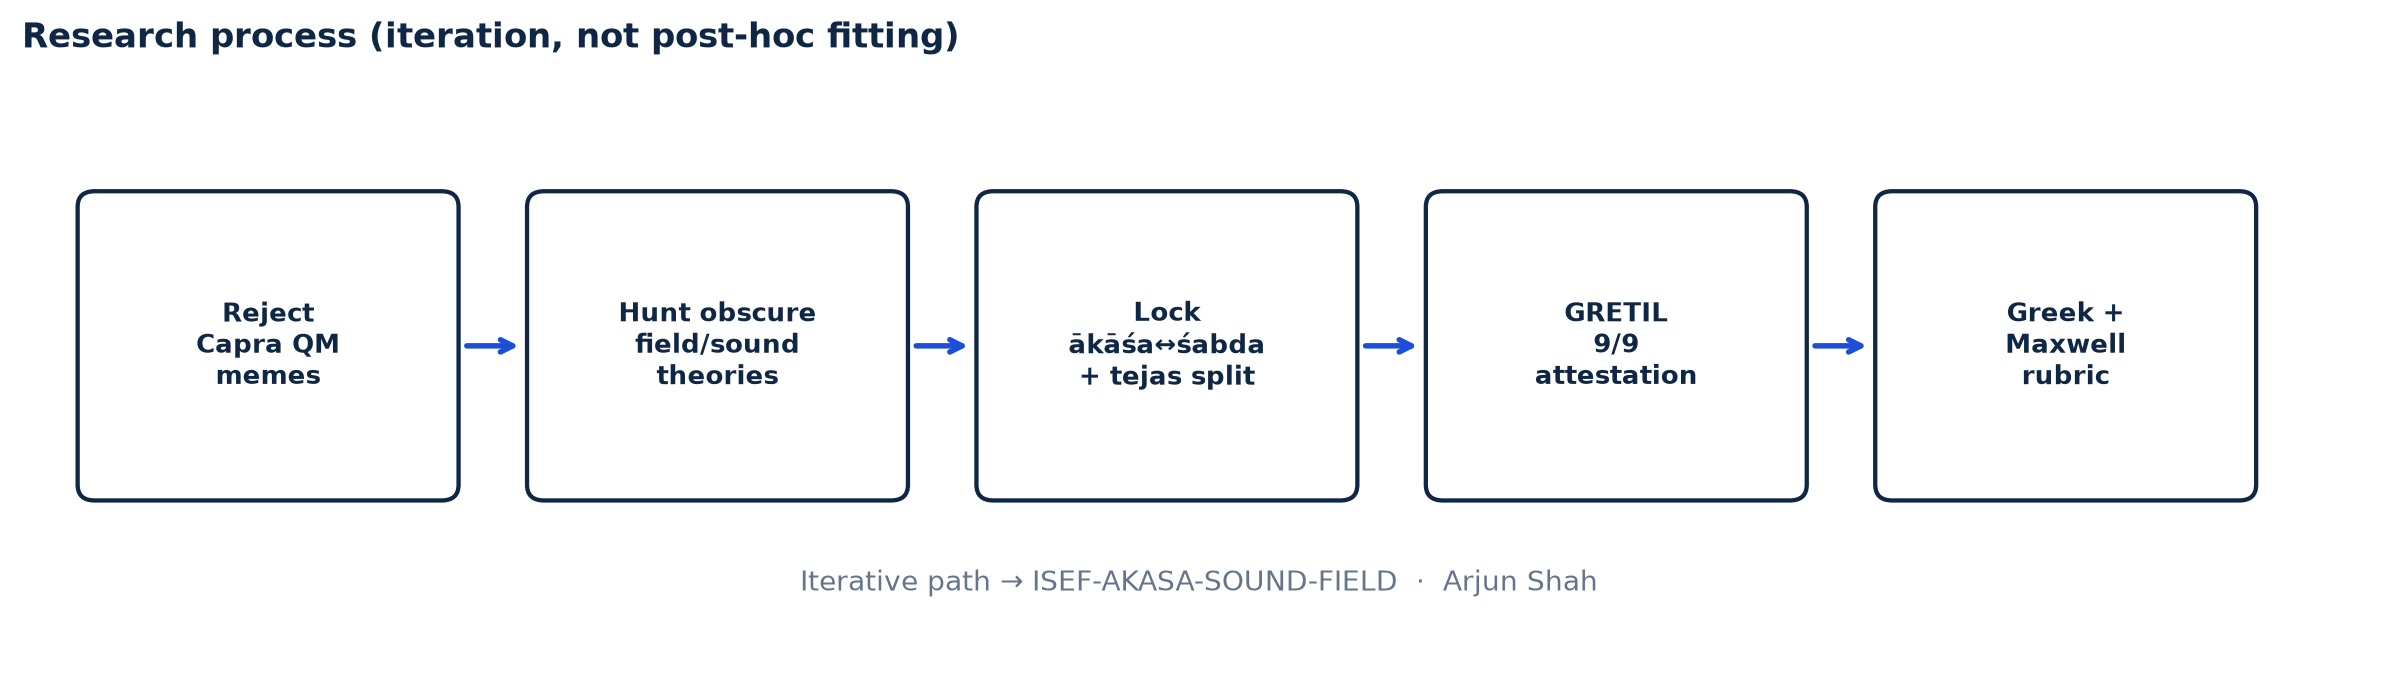
\includegraphics[width=\linewidth]{figures/fig42_isef_process.png}
\caption{Research progression from claim filtering to comparative testing.}
\label{fig:process}
\end{figure}

\begin{figure}[H]
\centering
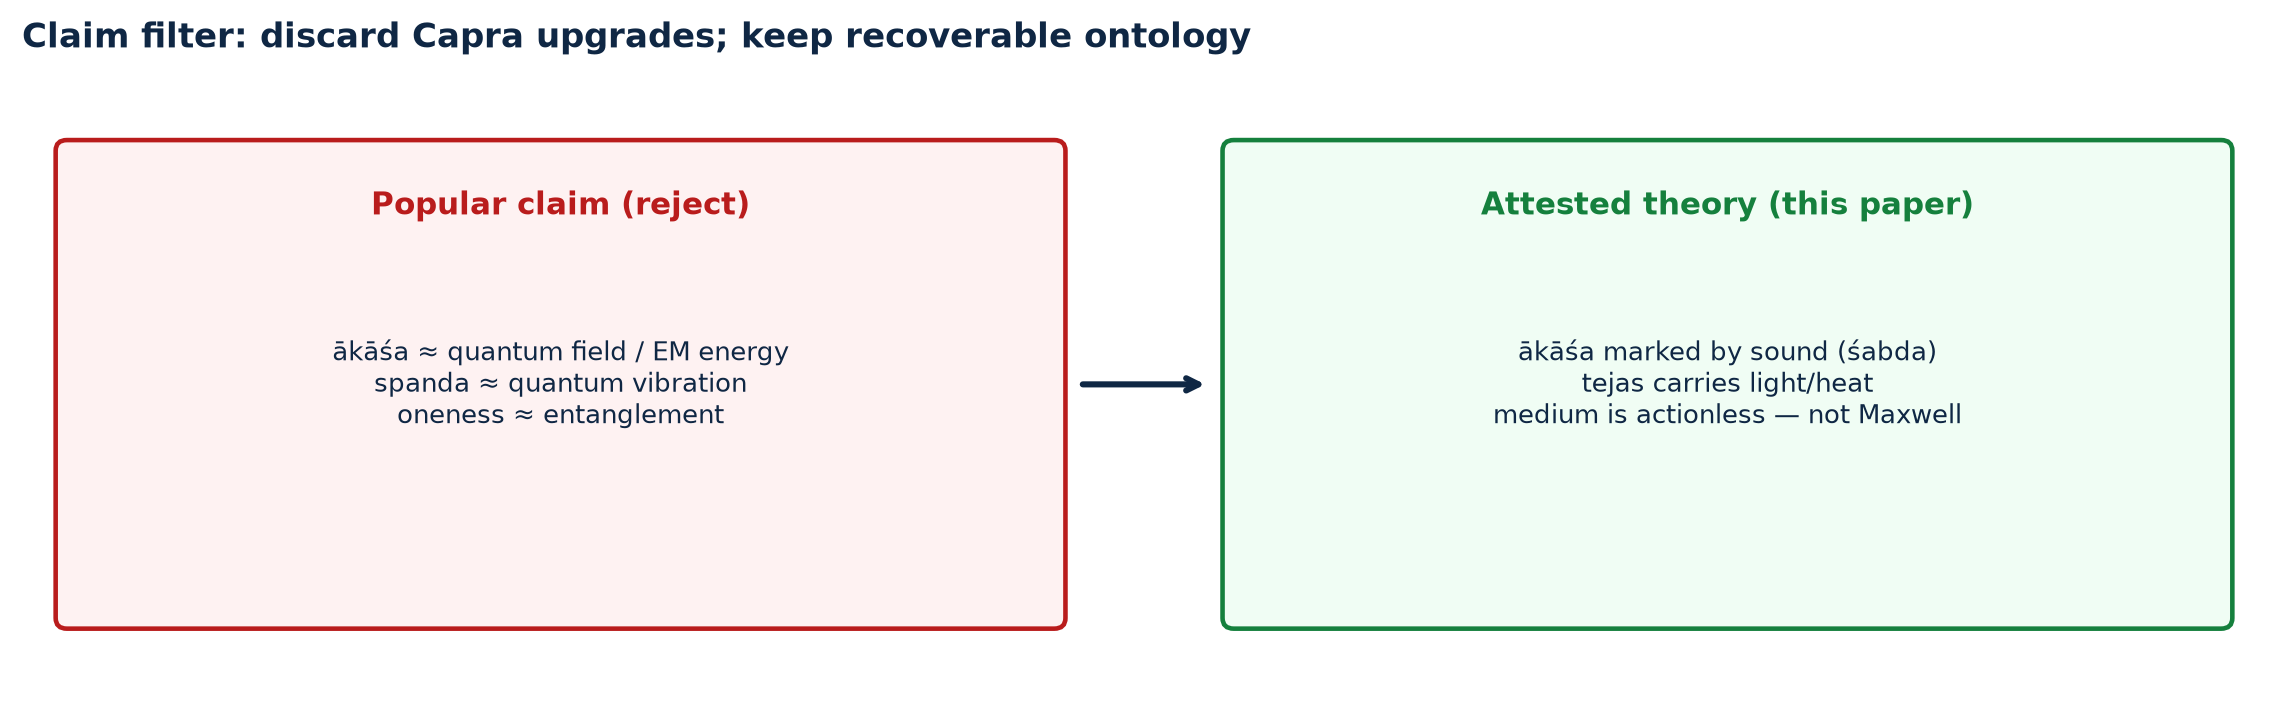
\includegraphics[width=0.92\linewidth]{figures/fig47_isef_claim_filter.png}
\caption{Claim filter: popular upgrades discarded; attested ontology retained.}
\label{fig:filter}
\end{figure}

\begin{figure}[H]
\centering
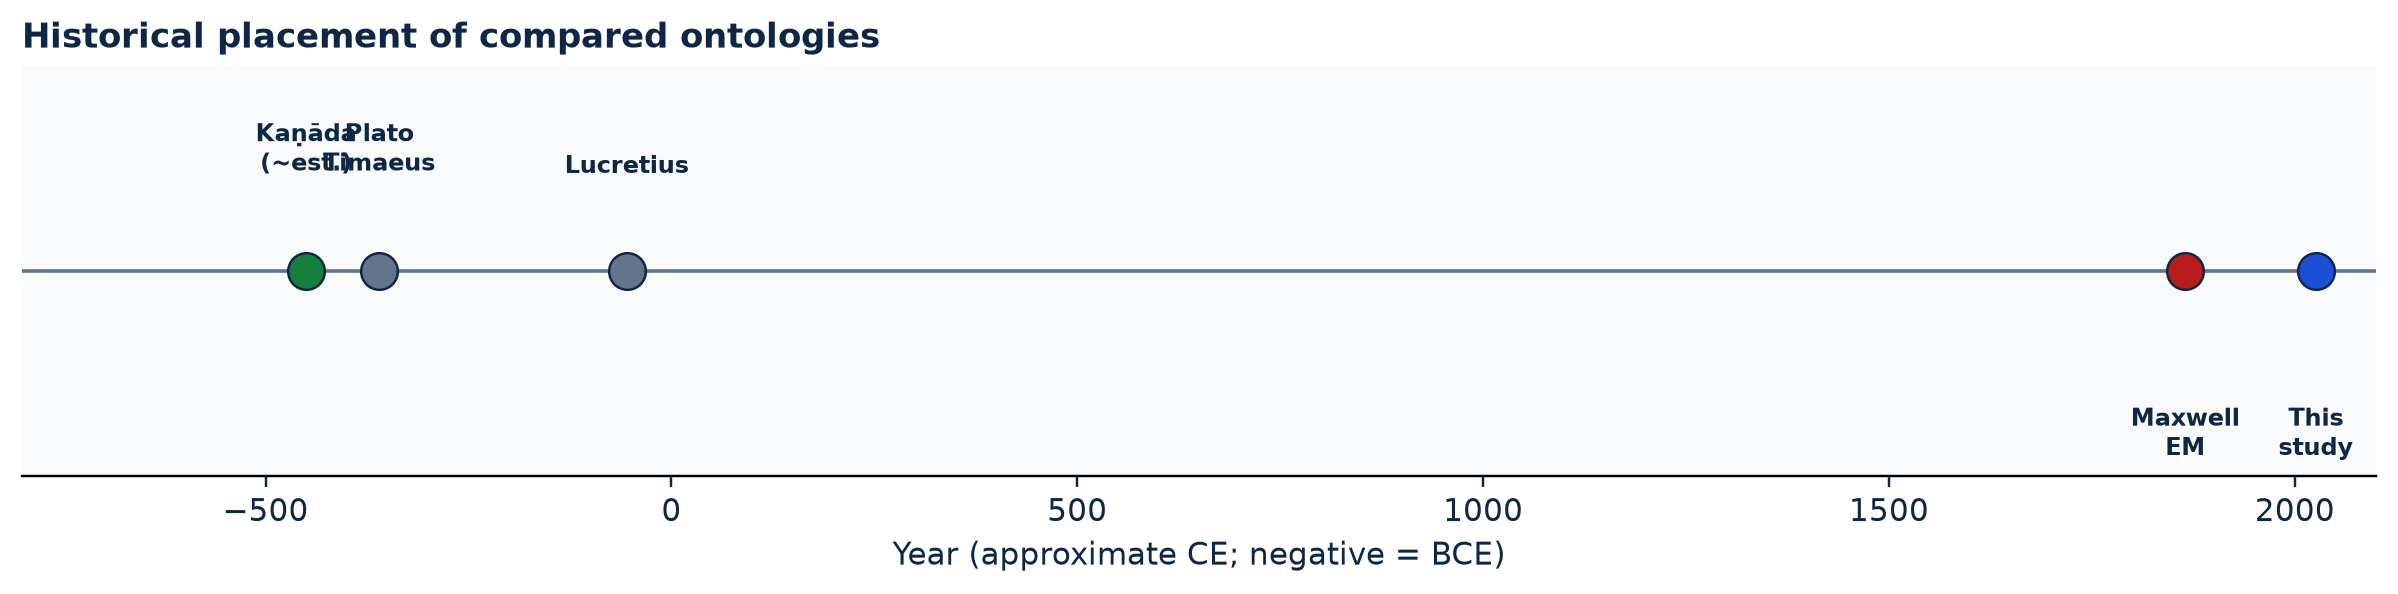
\includegraphics[width=\linewidth]{figures/fig43_isef_timeline.png}
\caption{Approximate historical placement of compared ontologies.}
\label{fig:timeline}
\end{figure}

% ========================= 4 METHODS =========================
\section{Materials and Methods}

\subsection{Materials}
\begin{itemize}
\item GRETIL digital \Vais{} Sutra (\Kanada), typed Unicode Sanskrit~\cite{gretil_vs}.
\item GRETIL \Pras{} \emph{Padarthadharmasamgraha} for commentarial replication.
\item Public-domain English panels in the RISHI-Q development corpus:
      Lucretius ($n=60$), Plato \emph{Timaeus} ($n=50$),
      Dao De Jing ($n=40$), Dhammapada ($n=40$).
\item Maxwell electromagnetism as textbook structural foil~\cite{jackson1999}.
\item Analysis scripts under \texttt{scripts/}
      (primary run, figure generation, and expansion v2).
\end{itemize}

\subsection{Procedure A --- Primary Attestation (T1--T9)}
The GRETIL file was downloaded and stripped of HTML.
Regular expressions indexed 369 sutra IDs of the form
\texttt{KVs\_x,y.z}.
Each checklist item required (i)~presence of the expected sutra ID(s) and
(ii)~pattern match on the Sanskrit body
(including compact match because GRETIL often omits spaces).
No manuscript OCR was performed.

Full item definitions appear in Appendix~\ref{app:T}.

\subsection{Procedure B --- Maxwell Confrontation (M1--M5)}
Each Maxwell item was scored present/absent in the attested \Vais{} ontology.
Absence was predicted a priori from the operational seed.

\subsection{Procedure C --- Comparative Rubric Scoring}
Vectors in $\{0,1\}^6$ were assigned to six traditions.
\Vais{} scores follow primary attestation.
Maxwell scores follow textbook structure.
Lucretius and \emph{Timaeus} scores use scholarly overrides on PD English (keyword-only scoring misclassifies void as a positive sound-medium).
Dao De Jing and Dhammapada scores reflect absence of a \Vais-style sound-marked ether doctrine in those PD panels.
Hamming distance $d(u,v)=\sum_i \mathbf{1}[u_i\neq v_i]$ summarizes pairwise divergence.

\subsection{Procedure D --- Commentarial Replication (C1--C6)}
Six propositions were scored on GRETIL \Pras{} text: \akasa{} listed; \sabda{} among \akasa{} qualities; \sabda{} as inferential mark; ear as nabhas-region; tejas named; all-pervasiveness / great magnitude.

\subsection{Procedure E --- Descriptive Nulls}
Under the null that each tradition independently draws R2$\sim$Bernoulli($1/2$),
\[
P(\text{exactly one R2$=1$ and it is \Vais})=\frac{1}{2^6}=\frac{1}{64}=0.015625.
\]
Separately, among all $2^6=64$ binary 6-vectors, the fraction with Hamming distance to Maxwell $\ge 4$ was computed ($0.344$).
These nulls are descriptive rarity readouts, not generative cultural models.

\subsection{Procedure F --- Novelty Audit}
Search terms targeted quantitative comparative packages linking \Vais{} sound-medium ontology to Maxwell and multi-civilization rubrics.
Findings were coded into ``exists qualitatively'' versus ``not found as open quantitative package.''

\subsection{Risk and Safety}
No human participants, vertebrate animals, or hazardous biological agents.
Public digital texts only.
Computational work on a personal computer.

\subsection{Data Analysis Plan}
Primary endpoints: T-pass count; C-pass count; M-hit count; R2 uniqueness; Hamming matrix; null probabilities.
All analyses are exploratory and fully reproducible from open scripts and JSON summaries under \texttt{results/exploratory/isef\_akasa\_sound\_field/}.

% ========================= 5 RESULTS =========================
\section{Results}

\subsection{Overview Board}
\begin{figure}[H]
\centering
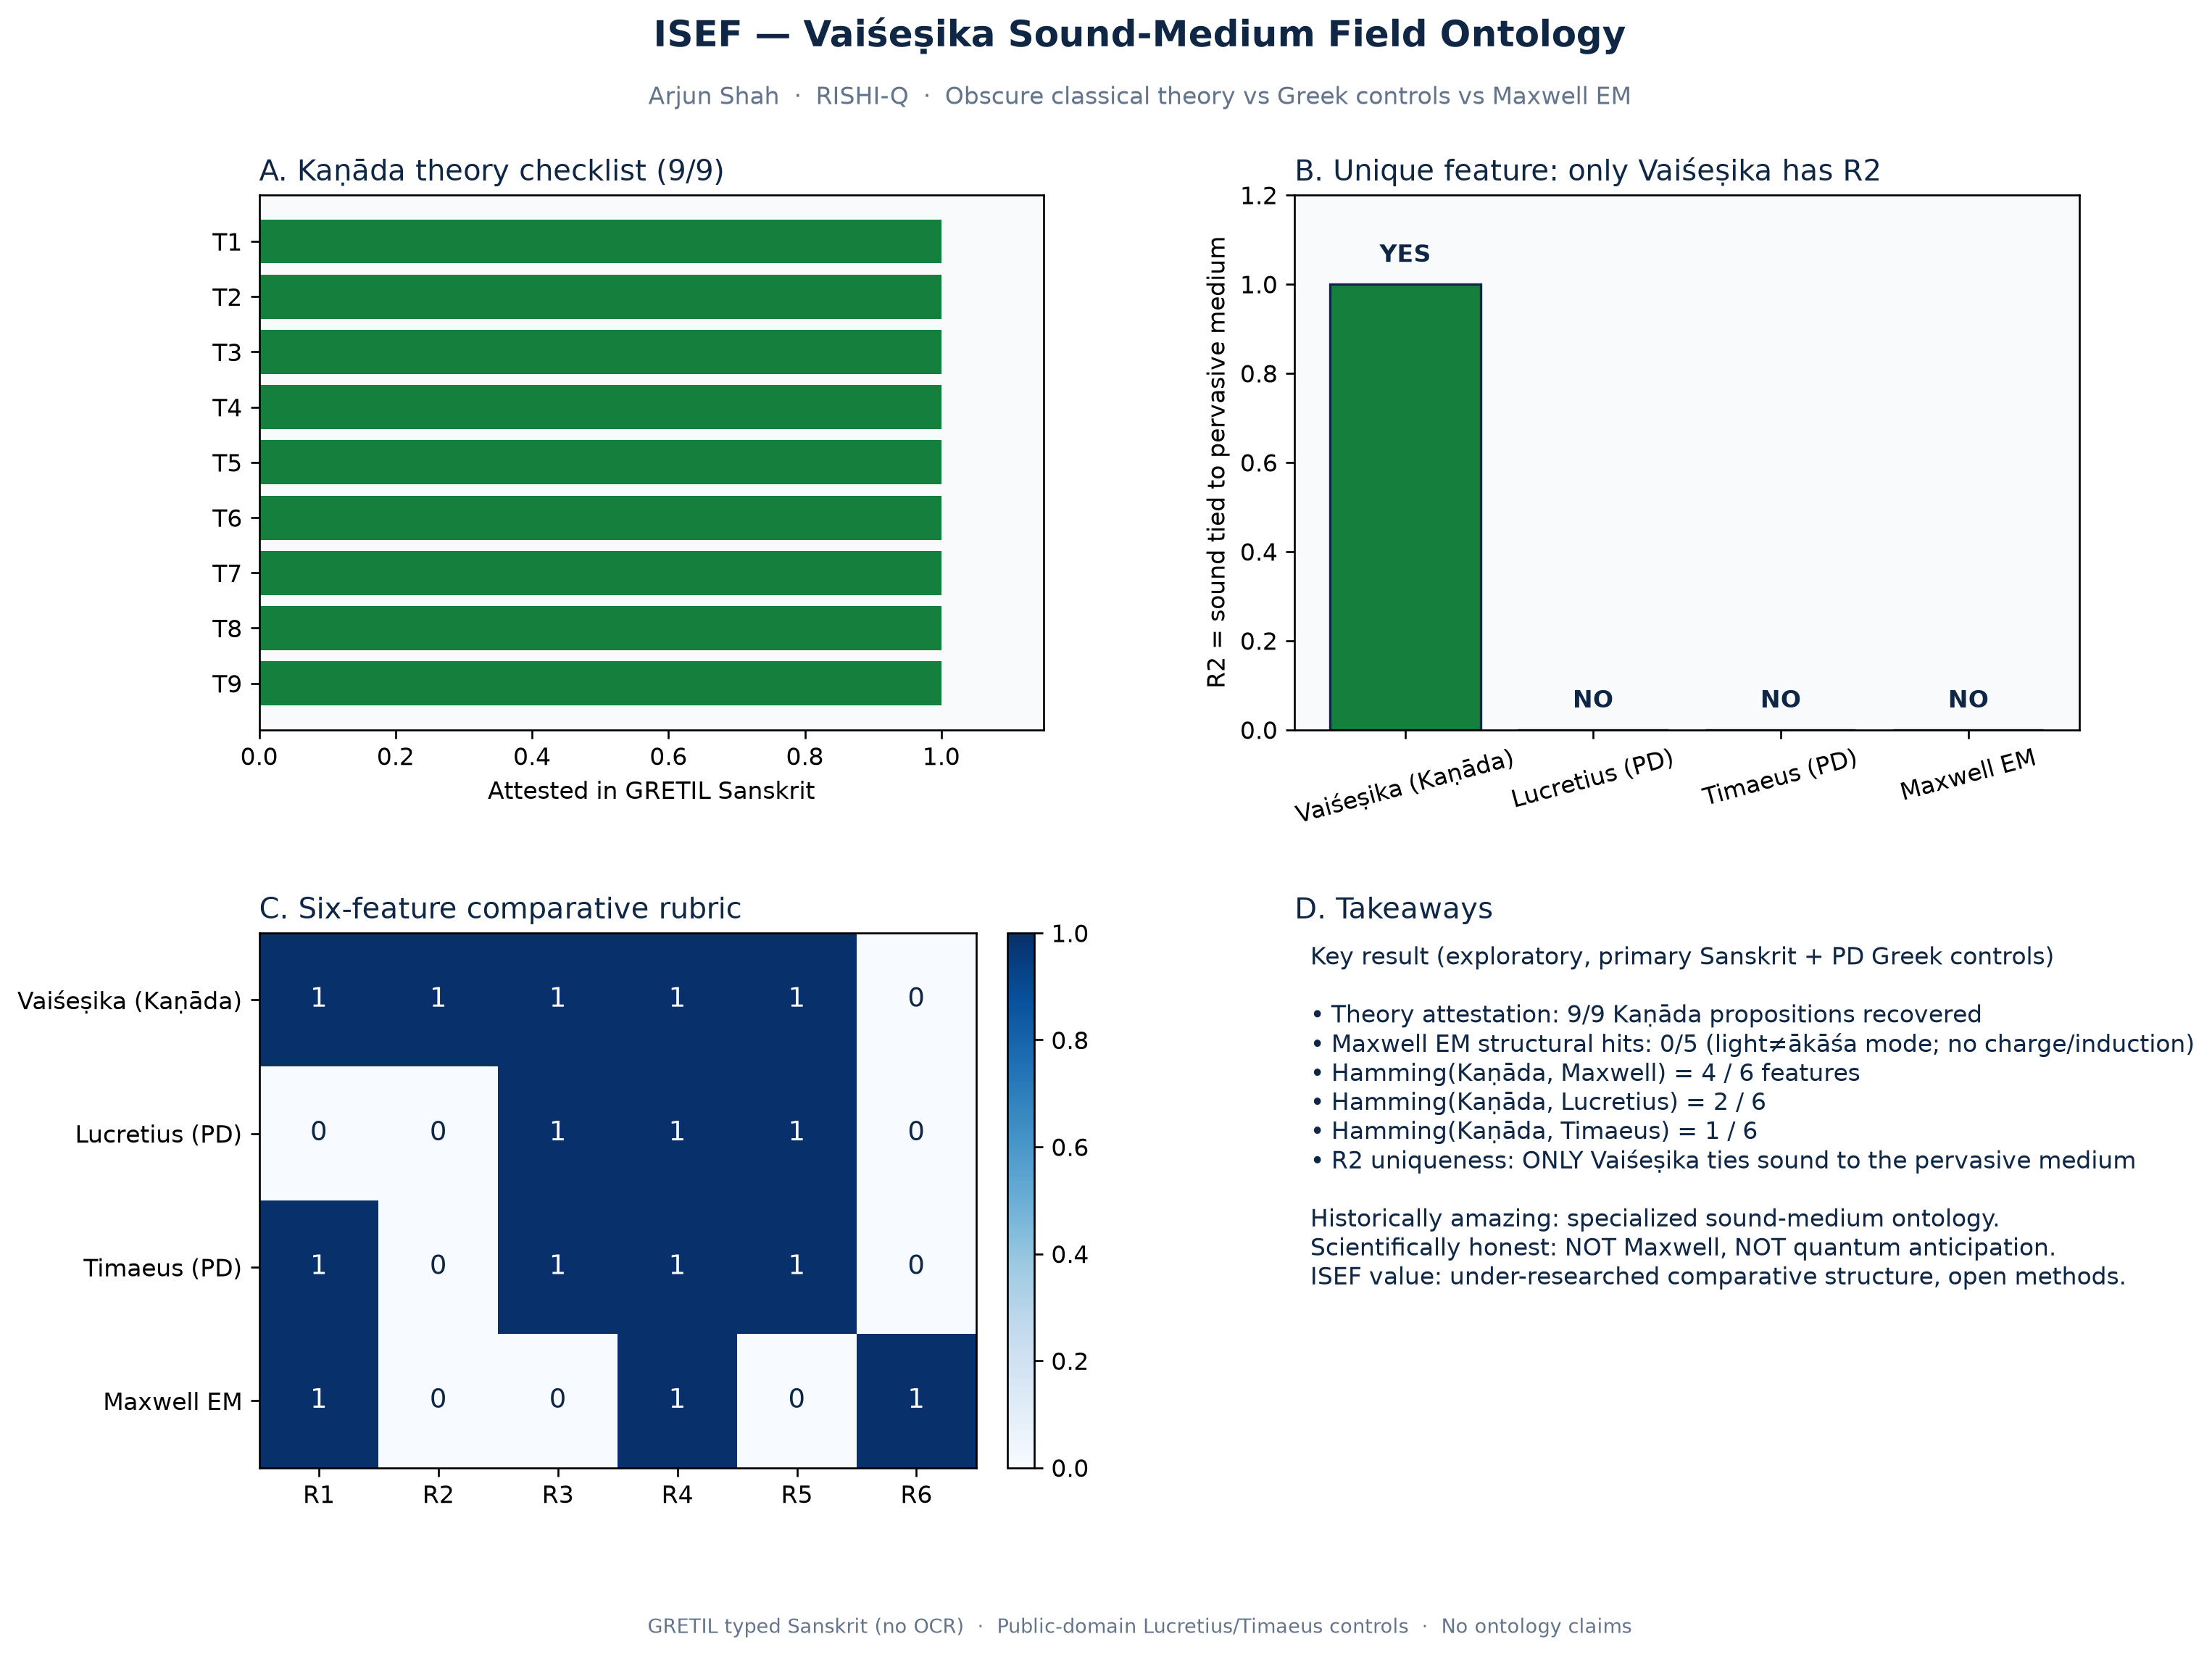
\includegraphics[width=\linewidth]{figures/fig41_isef_akasa_sound_field.png}
\caption{Primary results board: attestation, R2 uniqueness, rubric heatmap, takeaways.}
\label{fig:board}
\end{figure}

\subsection{H1 --- Primary Attestation: 9/9}
All nine theory propositions passed (Table~\ref{tab:Tfull}; Figure~\ref{fig:evidence}).

\begin{figure}[H]
\centering
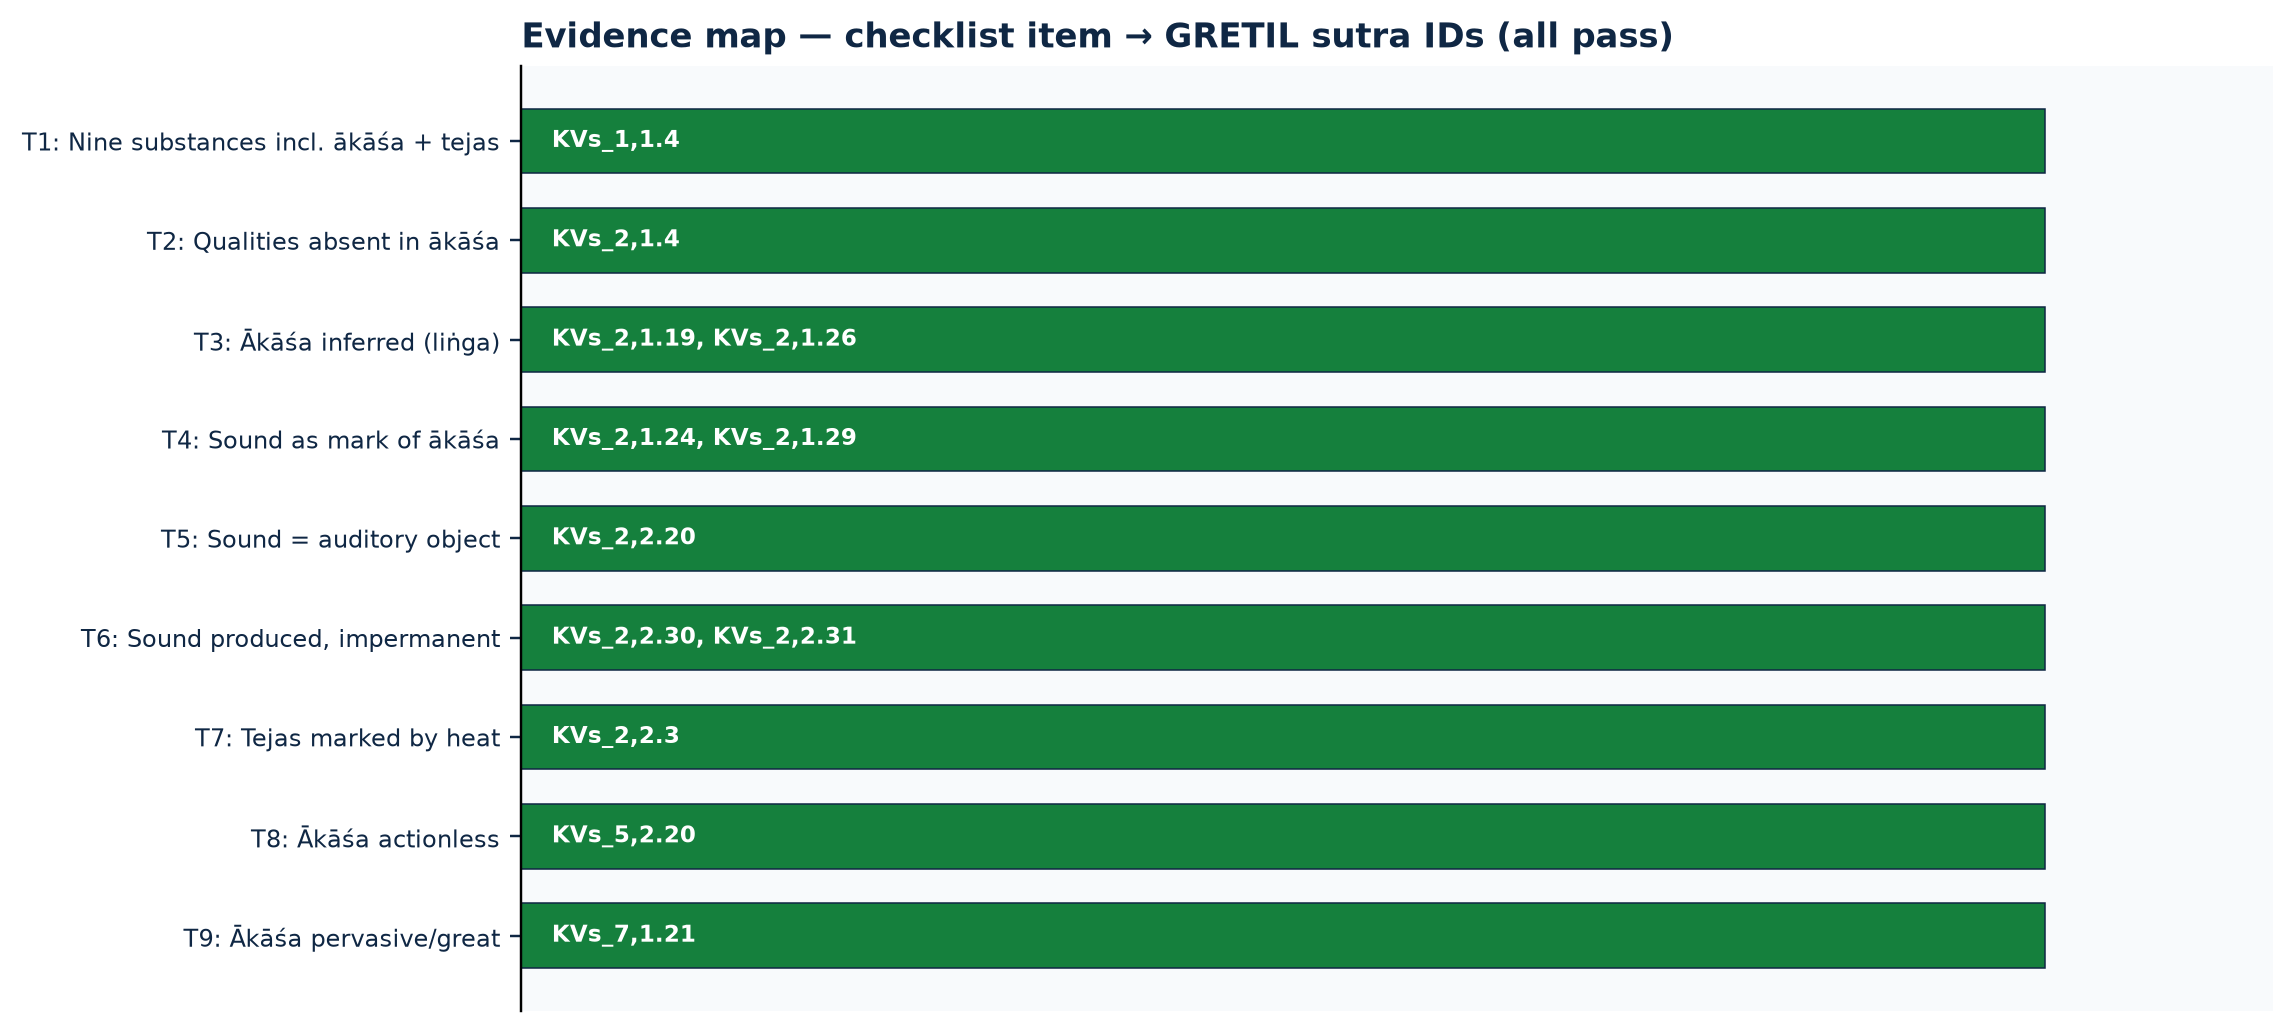
\includegraphics[width=\linewidth]{figures/fig46_isef_evidence.png}
\caption{Evidence map: checklist item to GRETIL sutra IDs (all pass).}
\label{fig:evidence}
\end{figure}

\begin{table}[H]
\centering
\caption{Complete primary attestation checklist (T1--T9).}
\label{tab:Tfull}
\begin{tabular}{@{}clp{6.2cm}l@{}}
\toprule
\textbf{ID} & \textbf{Pass} & \textbf{Claim} & \textbf{Sutra IDs} \\
\midrule
T1 & Yes & Nine substances incl.\ \akasa{} + tejas & KVs 1.1.4 \\
T2 & Yes & Qualities absent in \akasa & KVs 2.1.4 \\
T3 & Yes & \akasa{} inferred (liṅga) & KVs 2.1.19, 2.1.26 \\
T4 & Yes & Sound as mark of \akasa & KVs 2.1.24, 2.1.29 \\
T5 & Yes & Sound $=$ auditory object & KVs 2.2.20 \\
T6 & Yes & Sound produced, impermanent & KVs 2.2.30--31 \\
T7 & Yes & Tejas marked by heat & KVs 2.2.3 \\
T8 & Yes & \akasa{} actionless & KVs 5.2.20 \\
T9 & Yes & \akasa{} pervasive/great & KVs 7.1.21 \\
\midrule
Total & \textbf{9/9} & & \\
\bottomrule
\end{tabular}
\end{table}

\subsection{H2 --- Maxwell Confrontation: 0/5}
\begin{table}[H]
\centering
\caption{Maxwell structural confrontation (M1--M5).}
\label{tab:M}
\begin{tabular}{@{}clp{8.8cm}@{}}
\toprule
\textbf{ID} & \textbf{Found?} & \textbf{Item} \\
\midrule
M1 & No & Light as mode of same pervasive medium \\
M2 & No & Sound not defining quality of EM medium (ontology does the opposite) \\
M3 & No & Unified luminous + non-luminous radiation \\
M4 & No & Charge / induction / inverse-square law \\
M5 & No & Dynamical evolving field equations \\
\midrule
Total & \textbf{0/5} & \\
\bottomrule
\end{tabular}
\end{table}

\subsection{H3 --- Comparative Rubric and Uniqueness}
\begin{figure}[H]
\centering
\begin{minipage}{0.48\linewidth}
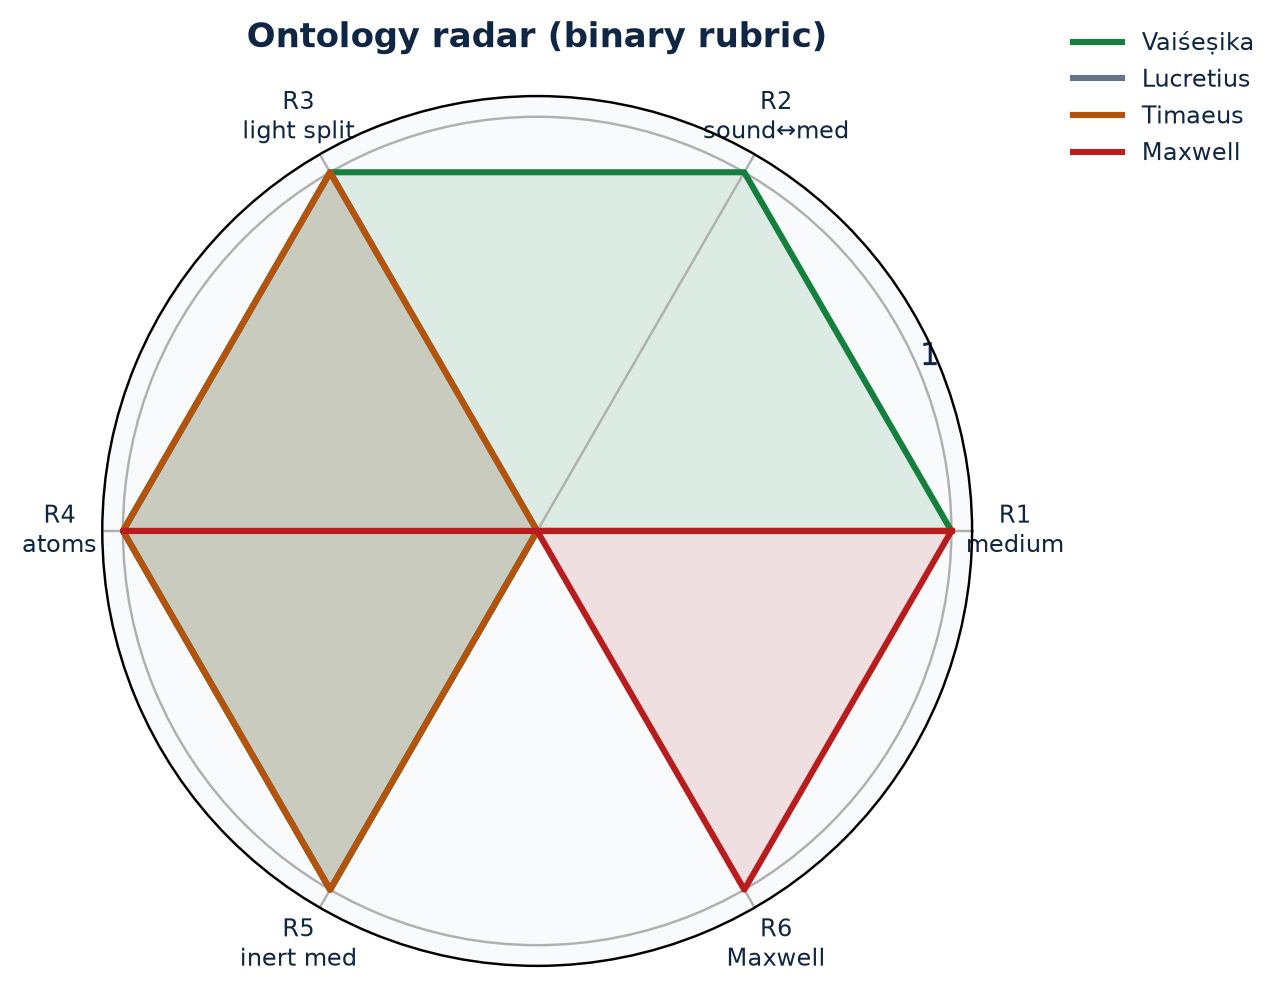
\includegraphics[width=\linewidth]{figures/fig44_isef_radar.png}
\end{minipage}\hfill
\begin{minipage}{0.48\linewidth}
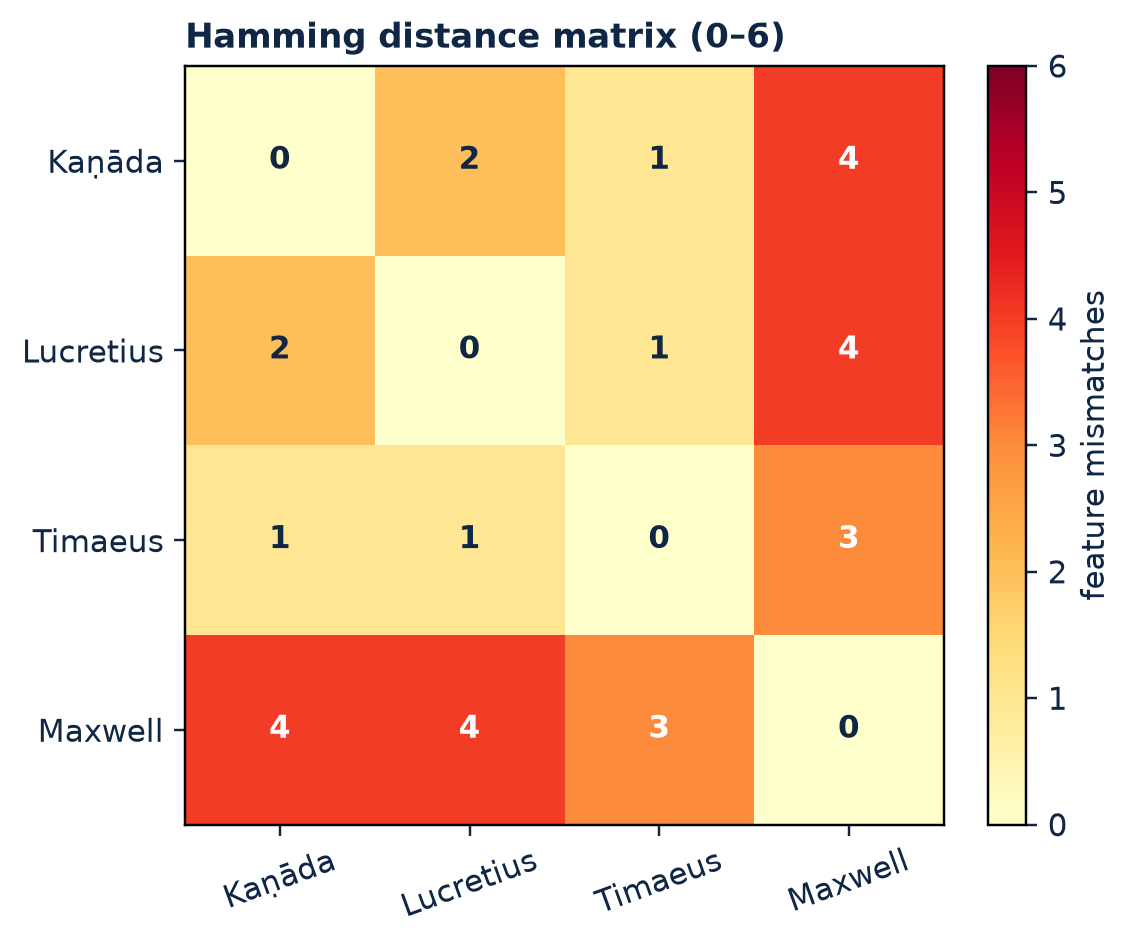
\includegraphics[width=\linewidth]{figures/fig45_isef_distance.png}
\end{minipage}
\caption{Left: ontology radar. Right: Hamming distance matrix.}
\label{fig:radar_dist}
\end{figure}

\begin{table}[H]
\centering
\caption{Six-tradition feature vectors (order R1--R6) and R2.}
\label{tab:vectors}
\begin{tabular}{@{}lccccccc@{}}
\toprule
\textbf{Tradition} & R1 & R2 & R3 & R4 & R5 & R6 & \textbf{R2} \\
\midrule
\Vais & 1 & 1 & 1 & 1 & 1 & 0 & \textbf{1} \\
Lucretius & 0 & 0 & 1 & 1 & 1 & 0 & 0 \\
\emph{Timaeus} & 1 & 0 & 1 & 1 & 1 & 0 & 0 \\
Dao De Jing & 1 & 0 & 0 & 0 & 1 & 0 & 0 \\
Dhammapada & 0 & 0 & 0 & 0 & 0 & 0 & 0 \\
Maxwell EM & 1 & 0 & 0 & 1 & 0 & 1 & 0 \\
\bottomrule
\end{tabular}
\end{table}

\begin{table}[H]
\centering
\caption{Selected Hamming distances.}
\label{tab:ham}
\begin{tabular}{@{}lc@{}}
\toprule
\textbf{Pair} & \textbf{Distance / 6} \\
\midrule
\Kanada{}--Maxwell & 4 \\
Lucretius--Maxwell & 4 \\
\emph{Timaeus}--Maxwell & 3 \\
\Kanada{}--Lucretius & 2 \\
\Kanada{}--\emph{Timaeus} & 1 \\
\bottomrule
\end{tabular}
\end{table}

Only \Vais{} scores R2 $=1$.
\Kanada{} is nearest Greek medium/receptacle structure on gross features, yet far from Maxwell on unification and dynamics.

\subsection{H4 --- \Pras{} Replication: 6/6}
\begin{table}[H]
\centering
\caption{Commentarial replication checklist.}
\label{tab:C}
\begin{tabular}{@{}clp{8.5cm}@{}}
\toprule
\textbf{ID} & \textbf{Pass} & \textbf{Claim} \\
\midrule
C1 & Yes & \akasa{} in substance list \\
C2 & Yes & \sabda{} among \akasa{} qualities \\
C3 & Yes & \sabda{} as inferential mark \\
C4 & Yes & Ear as nabhas / ether-region \\
C5 & Yes & Tejas as distinct substance \\
C6 & Yes & All-pervasiveness / great magnitude \\
\midrule
Total & \textbf{6/6} & \\
\bottomrule
\end{tabular}
\end{table}

\subsection{Expansion Board, Nulls, Ontology Graph, Novelty}
\begin{figure}[H]
\centering
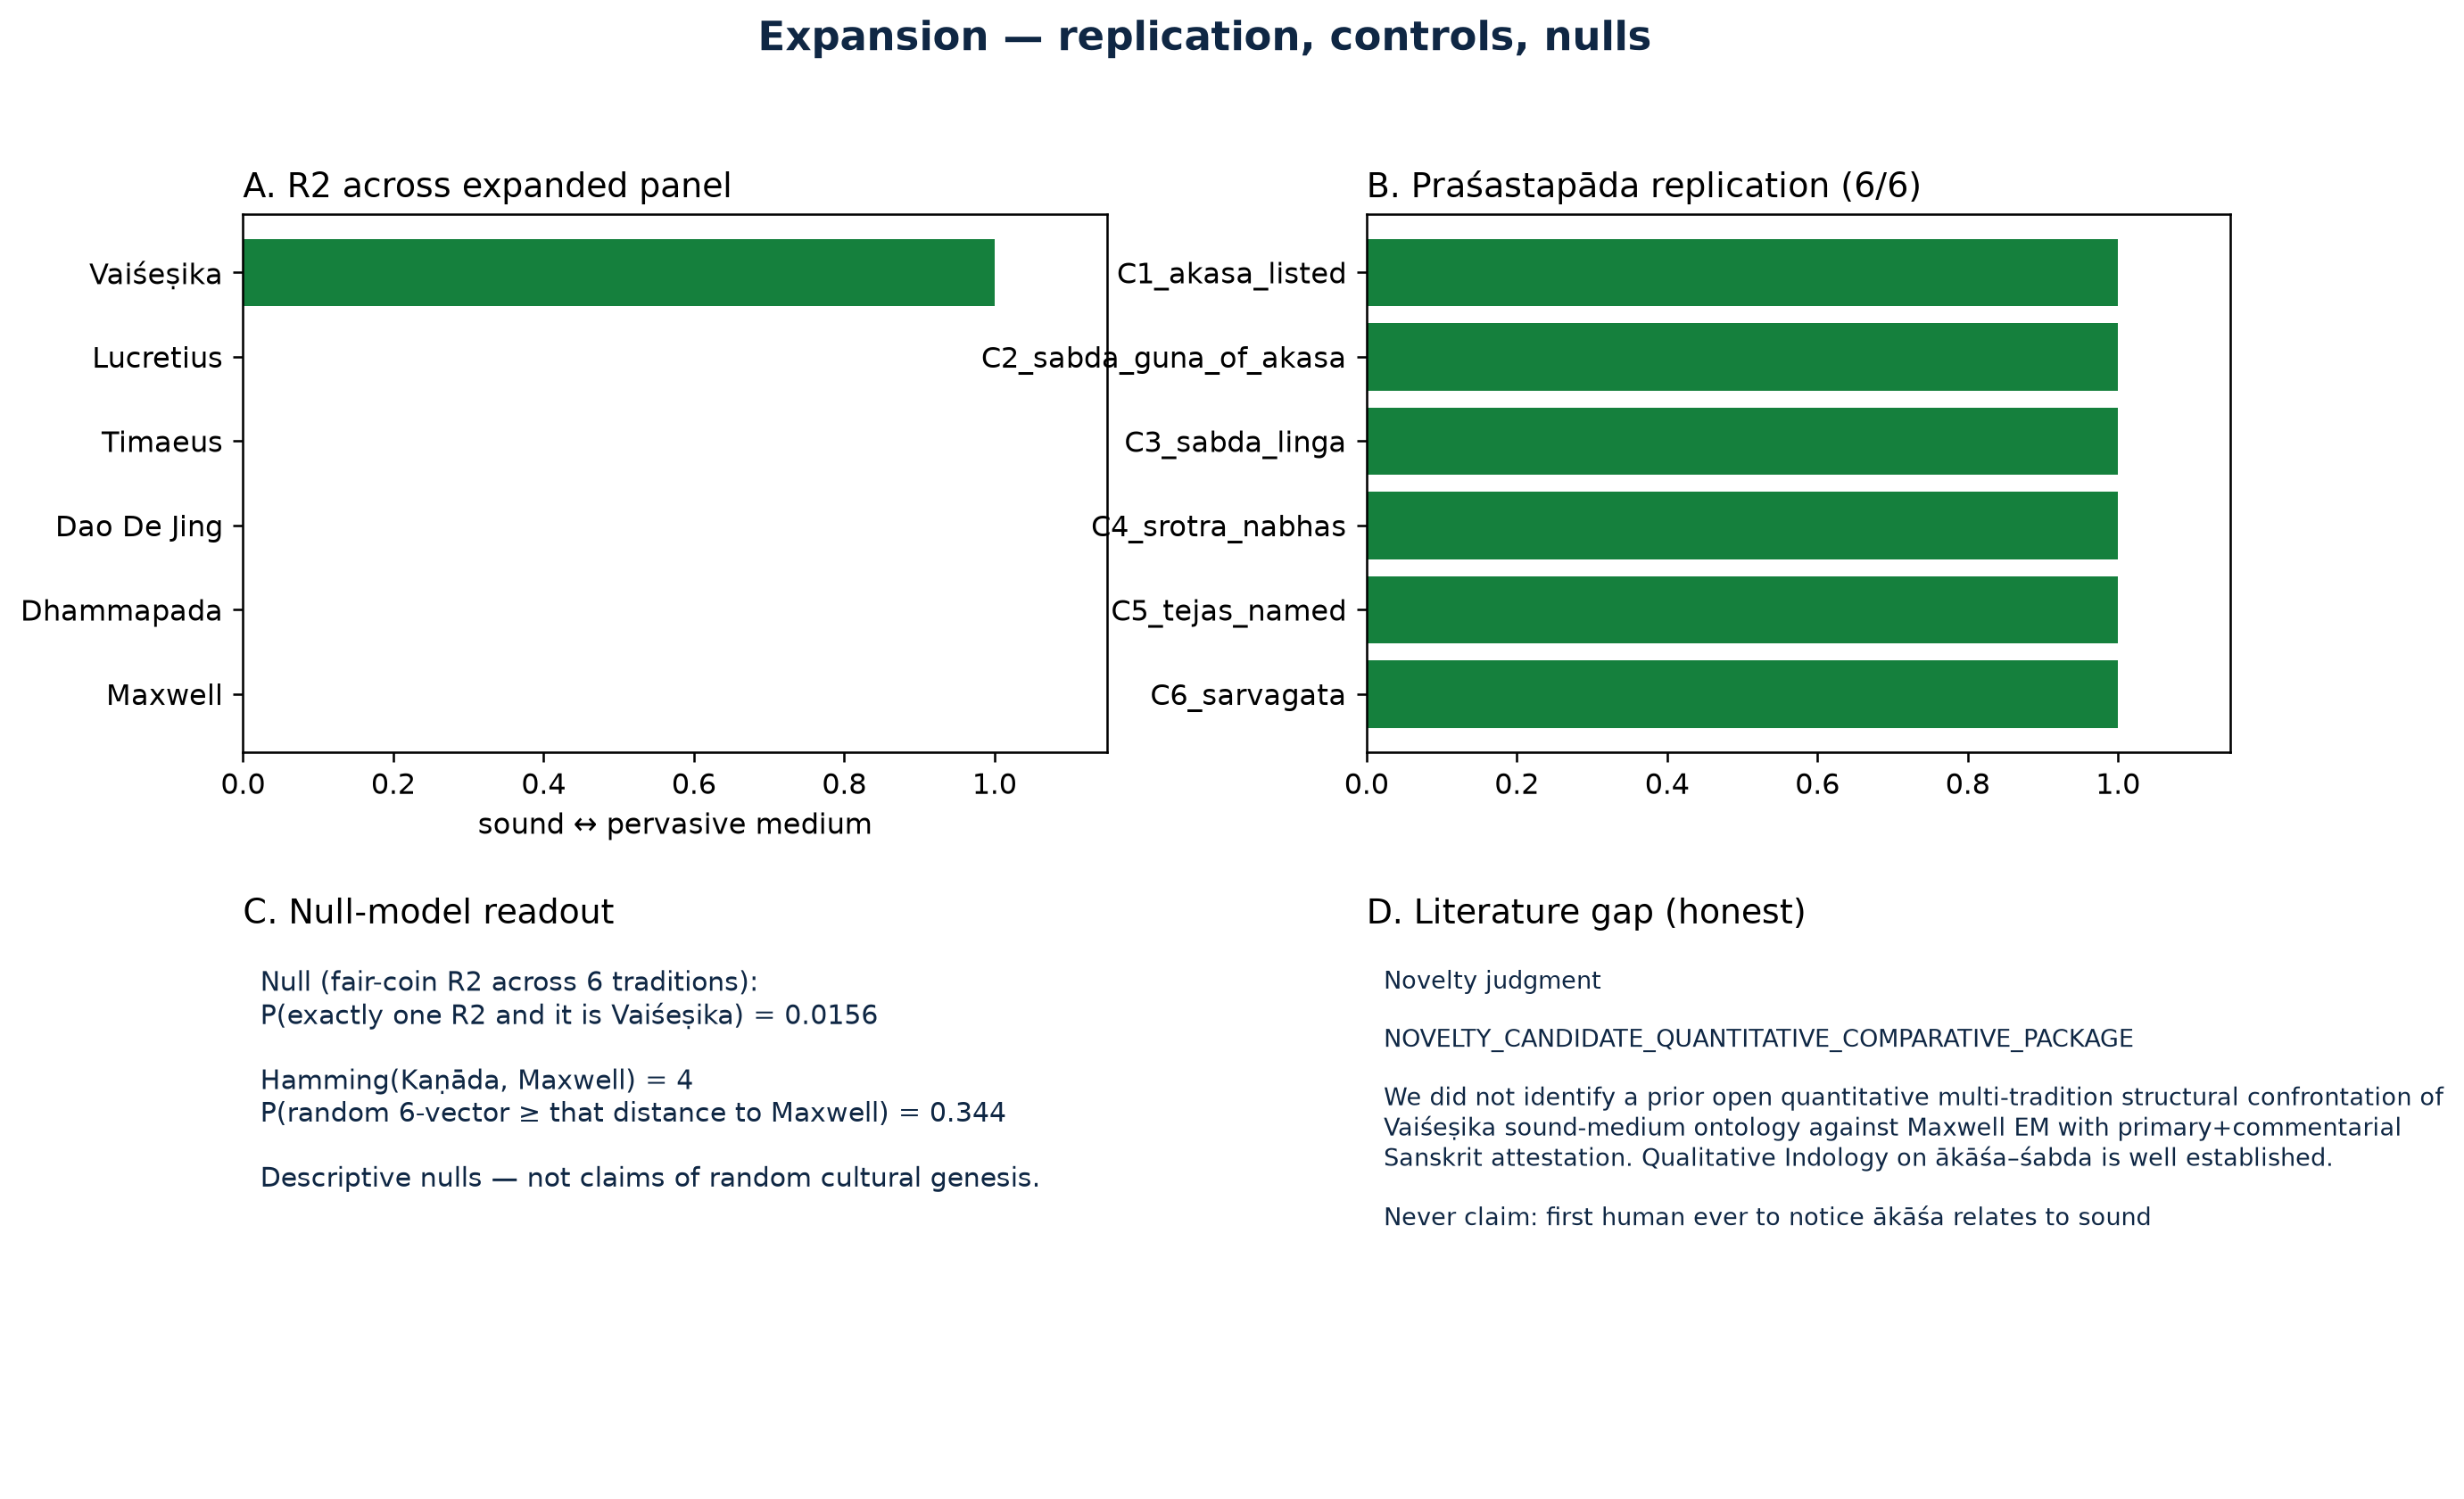
\includegraphics[width=\linewidth]{figures/fig49_isef_expansion_board.png}
\caption{Expansion board: R2 panel, \Pras{} replication, nulls, novelty judgment.}
\label{fig:exp}
\end{figure}

\textbf{Null readout.}
$P(\text{exactly one R2 and it is \Vais})=1/64=0.015625$ under independent fair-coin R2 draws.
$P(d(\cdot,\text{Maxwell})\ge 4)=0.344$ among all 6-bit vectors.

\begin{figure}[H]
\centering
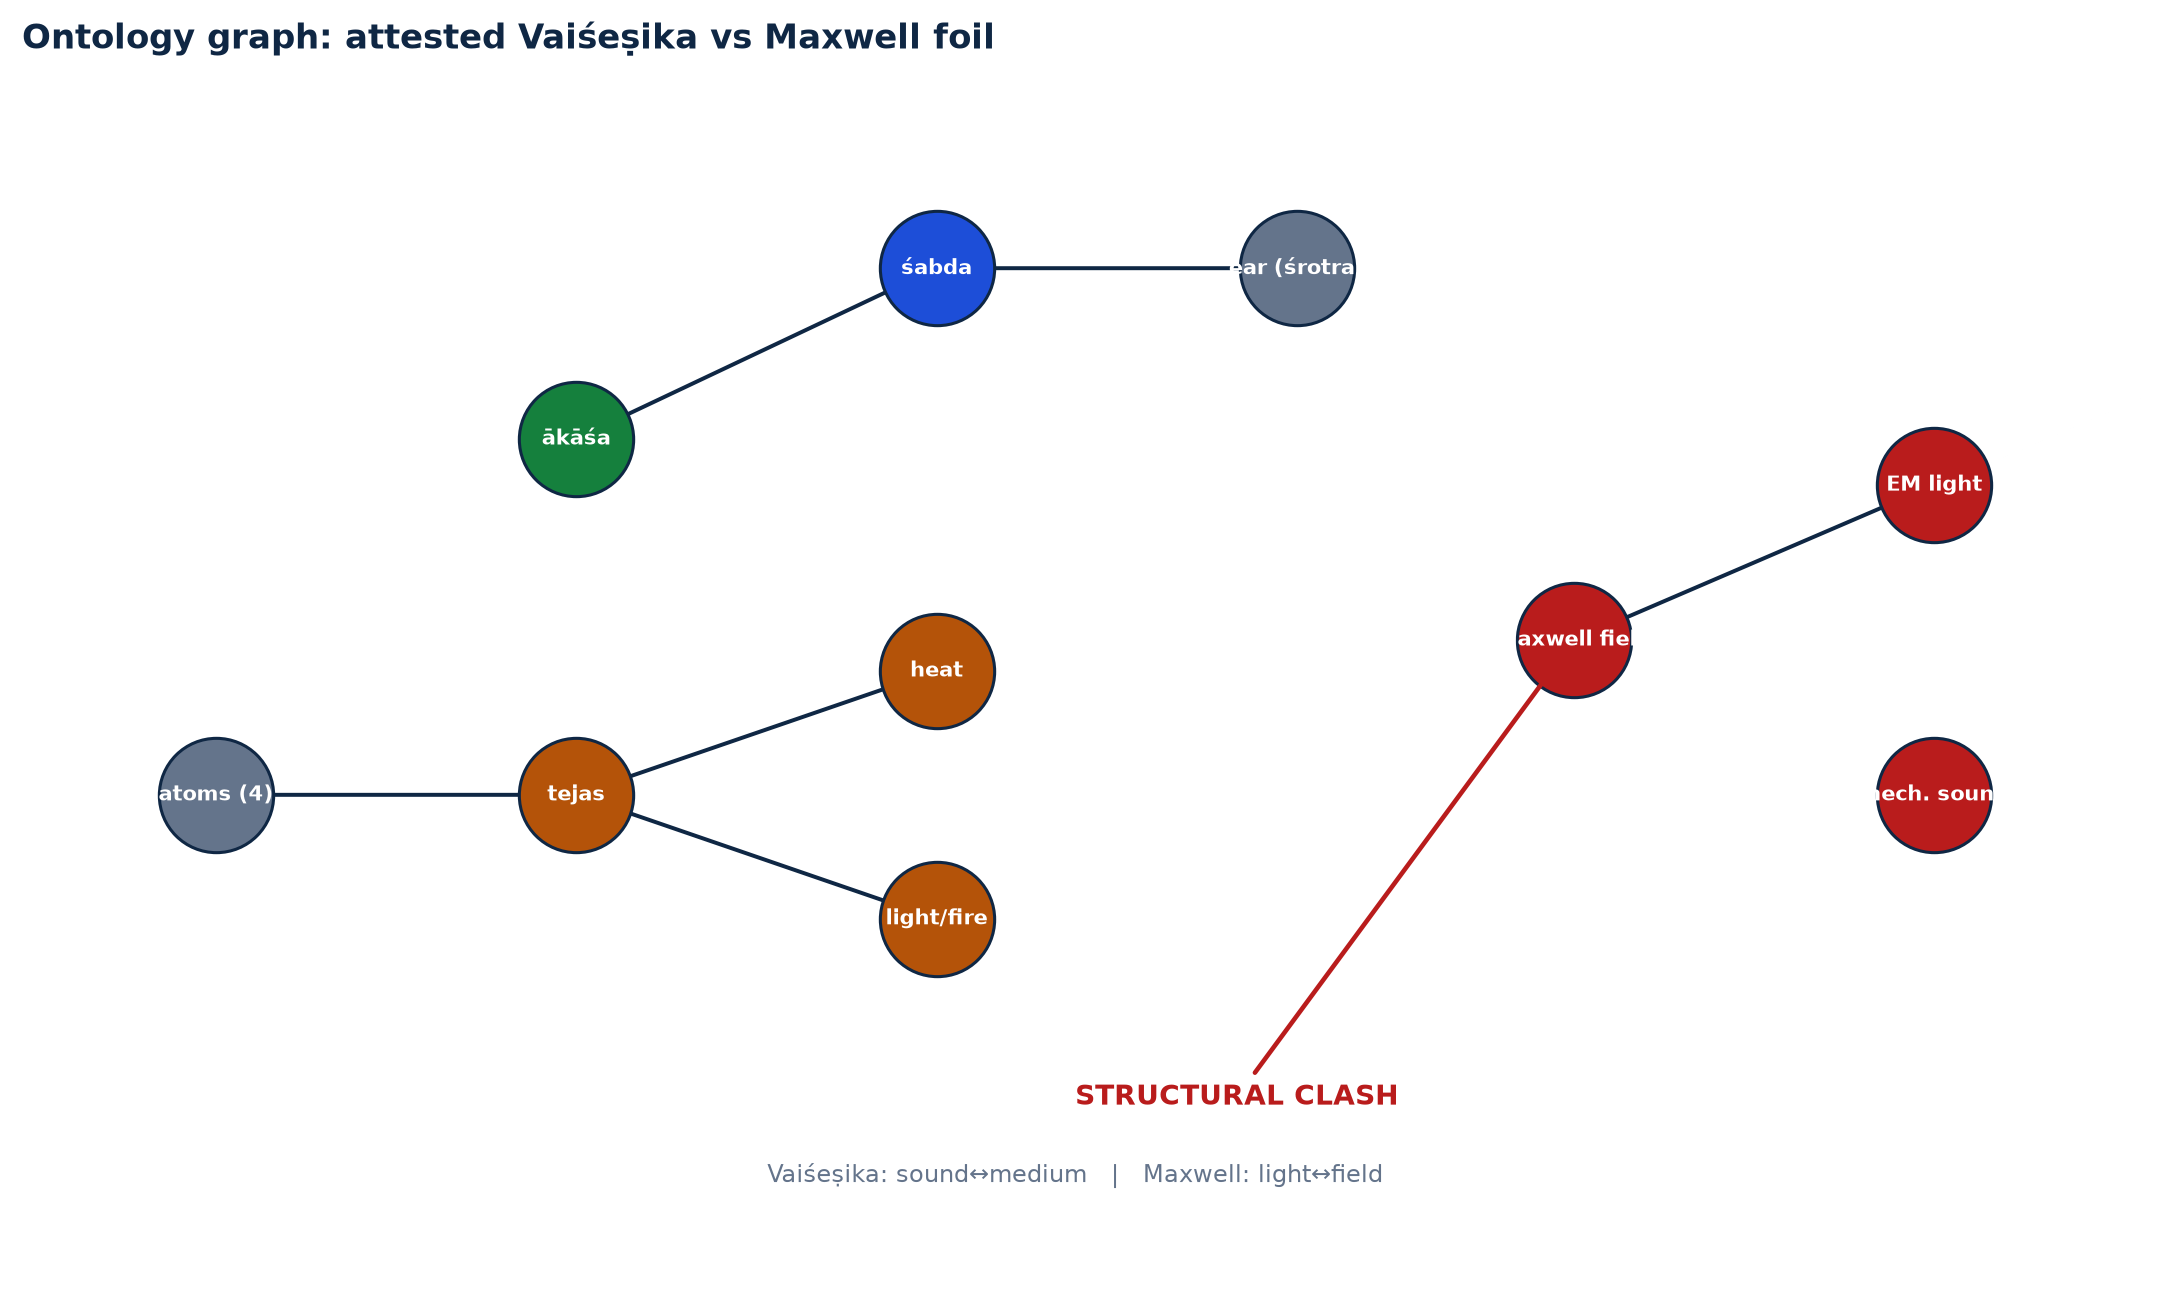
\includegraphics[width=0.90\linewidth]{figures/fig48_isef_ontology_graph.png}
\caption{Ontology graph: attested \Vais{} edges versus Maxwell foil.}
\label{fig:graph}
\end{figure}

\textbf{Novelty judgment.}
Qualitative Indology on \akasa{}--\sabda{} is established~\citep{halbfass1992,potter1977}.
An open quantitative multi-civilization package with primary+commentarial counts, Maxwell foil, nulls, and explicit refusal of Capra upgrades was not identified in search.
Never claim ``first human to notice sound relates to \akasa.''
Do claim a new open computational comparison instrument.

% ========================= 6 DISCUSSION =========================
\section{Discussion}

\subsection{Interpretation of Supported Hypotheses}
H1--H4 were supported.
The historically impressive content is not secret Maxwellian physics; it is early formalization of a \emph{sensory-indexed medium}: a pervasive substance known through sound, with light/heat located elsewhere.
That is precise natural philosophy.
It is also why Maxwell confrontation fails cleanly: Maxwell indexes the field to electromagnetic radiation (including light), not to sound.

\subsection{Why R2 Matters}
Many traditions can score R1 (some pervasive medium or continuum talk).
R2 is stricter.
It asks whether sound is the special key to that medium.
On the six-tradition panel, only \Vais{} passes.
That uniqueness is the comparative core of the paper.

\subsection{Value of the Negative Maxwell Result}
In ISEF and professional science, a negative that follows from a preregistered-style checklist is a result.
Fabricating EM anticipation would be the failure mode.
Reporting 0/5 Maxwell hits, with open methods, is the honest product.

\subsection{Relation to Broader RISHI-Q Program}
Prior Capra autopsy work showed Level-III quantum failure on Vedānta PD text.
This paper is the constructive sequel: pick an obscure classical doctrine that \emph{does} have sharp structure, then test whether that structure is Maxwellian.
Answer: no---but the doctrine is real and under-discussed in popular ``ancient science'' discourse.

\subsection{Limitations (Detailed)}
\begin{enumerate}
\item GRETIL is a reference digital edition, not a fully proofread critical edition for every sandhi.
\item Greek/Chinese/Buddhist scores use public-domain English with scholarly overrides; a Sanskrit/Greek/Chinese specialist panel could refine coding.
\item Rubric features are coarse binary summaries of rich philosophies.
\item Null models are descriptive, not causal historical models.
\item No laboratory acoustics or magnetometry component is included.
\item Later Nyāya--\Vais{} commentarial diversity beyond \Pras{} is not exhaustively scored.
\end{enumerate}

\subsection{Threats to Validity and Mitigations}
\begin{itemize}
\item \textbf{Parse artifact:} mitigated by \Pras{} 6/6 replication.
\item \textbf{Keyword false friends:} mitigated by scholarly overrides and explicit notes in code.
\item \textbf{Confirmation bias:} mitigated by freezing Maxwell items that predict failure, and by reporting negatives prominently.
\item \textbf{Novelty overclaim:} mitigated by explicit ``never claim first notice of \akasa{}--sound.''
\end{itemize}

\subsection{Future Work}
\begin{enumerate}
\item Add Jain and technical Buddhist sound doctrines as further Indian controls.
\item Score additional commentaries for R2 stability.
\item Human specialist audit of rubric cells.
\item Optional later laboratory study (structured sound protocols with optical/EM twins) only after textual freeze.
\end{enumerate}

% ========================= 7 CONCLUSIONS =========================
\section{Conclusions}
\begin{enumerate}
\item \Vais{} encodes a recoverable sound-marked pervasive medium (primary attestation \textbf{9/9}).
\item Core claims replicate in \Pras{} (\textbf{6/6}).
\item The ontology fails Maxwell structural features (\textbf{0/5}).
\item Feature R2 is unique across a six-tradition panel; fair-coin null $P=1/64$.
\item The ISEF contribution is an open multi-civilization falsification-and-comparison package, not a claim of ancient electromagnetic or quantum discovery.
\end{enumerate}

\section*{Acknowledgments}
\addcontentsline{toc}{section}{Acknowledgments}
GRETIL / SUB Göttingen; Halbfass and Potter for \Vais{} scholarship; public-domain Lucretius and \emph{Timaeus} panels used as controls.

\section*{Data and Code Availability}
\addcontentsline{toc}{section}{Data and Code Availability}
\noindent
All analyses are reproducible from the RISHI-Q repository.
Run the primary attestation, figure-generation, and expansion scripts in the \texttt{scripts} folder, then compile this paper with tectonic.
Machine-readable JSON summaries and novelty notes are in the exploratory results folder; figures are in \texttt{paper/figures}.

\section*{Ethics Statement}
\addcontentsline{toc}{section}{Ethics Statement}
No human subjects, vertebrate animals, or potentially hazardous biological agents were used.
All textual sources are public digital editions or public-domain translations.
This work is not medical or engineering advice.
Any AI assistance was limited to drafting and engineering support; scientific claims, analyses, and final wording are the author's responsibility.

\section*{Author}
\addcontentsline{toc}{section}{Author}
Arjun Shah designed the study, implemented the software, performed the analyses, generated the figures, and wrote the paper.

\renewcommand{\refname}{Bibliography}
\addcontentsline{toc}{section}{Bibliography}
\bibliographystyle{plainnat}
\bibliography{references}

\newpage
\appendix
\section{Appendix A: Primary Checklist Definitions}
\label{app:T}
\noindent\textbf{T1.} Substance list includes both \akasa{} and tejas as distinct entries (KVs 1.1.4).\\
\textbf{T2.} Ordinary sense-qualities do not exist in \akasa{} (KVs 2.1.4).\\
\textbf{T3.} \akasa{} is established by inference / residual mark (KVs 2.1.19, 2.1.26).\\
\textbf{T4.} Sound functions as distinctive mark in \akasa{} inference (KVs 2.1.24, 2.1.29).\\
\textbf{T5.} Sound is defined as the object of hearing (KVs 2.2.20).\\
\textbf{T6.} Sound is produced (conjunction/disjunction) and impermanent (KVs 2.2.30--31).\\
\textbf{T7.} Tejas is marked by heat, separating light/fire substance from \akasa{} (KVs 2.2.3).\\
\textbf{T8.} \akasa{} is actionless / non-kinetic relative to dynamical field metaphors (KVs 5.2.20).\\
\textbf{T9.} \akasa{} is great / pervasive (KVs 7.1.21).

\section{Appendix B: Rubric Coding Notes}
\label{app:R}
\noindent\textbf{Lucretius:} R1$=0$ (void is absence, not a positive sound-medium); R2$=0$; R3$=1$; R4$=1$; R5$=1$; R6$=0$.\\
\textbf{Timaeus:} R1$=1$ (receptacle/space); R2$=0$; R3$=1$; R4$=1$; R5$=1$; R6$=0$.\\
\textbf{Dao De Jing PD:} R1$=1$ (process/way continuum talk); R2$=0$; R3$=0$; R4$=0$; R5$=1$; R6$=0$.\\
\textbf{Dhammapada PD:} all zeros on this natural-philosophy rubric (ethical verse panel).\\
\textbf{Maxwell:} R1$=1$; R2$=0$; R3$=0$ (light is the field); R4$=1$; R5$=0$; R6$=1$.

\section{Appendix C: Safe Groundbreaking Claim}
\label{app:claim}
\noindent
First open computational package combining (i)~GRETIL \Kanada{} attestation, (ii)~\Pras{} replication, (iii)~multi-civilization rubric including Greek/Chinese/Buddhist controls, (iv)~Maxwell foil, (v)~descriptive nulls on R2 uniqueness---while refusing Capra-style EM/QM anticipation claims.

\section{Appendix D: Figure Inventory}
\label{app:fig}
\begin{itemize}
\item Fig.~\ref{fig:process} --- research process
\item Fig.~\ref{fig:filter} --- claim filter
\item Fig.~\ref{fig:timeline} --- historical timeline
\item Fig.~\ref{fig:board} --- primary board
\item Fig.~\ref{fig:evidence} --- evidence map
\item Fig.~\ref{fig:radar_dist} --- radar + distances
\item Fig.~\ref{fig:exp} --- expansion board
\item Fig.~\ref{fig:graph} --- ontology graph
\end{itemize}

\section{Appendix E: Reproducibility Checklist}
\label{app:repro}
\begin{enumerate}
\item Clone / open RISHI-Q repository.
\item Run the three scripts listed under Data and Code Availability.
\item Confirm \texttt{summary.json} shows theory 9/9 and Maxwell 0/5.
\item Confirm \texttt{expansion\_v2.json} shows \Pras{} 6/6 and null $P=0.015625$.
\item Compile this paper with \texttt{tectonic isef\_report.tex}.
\end{enumerate}

\end{document}
